\begin{frame}
  \frametitle{Steady-state criticality simulation results}
     \begin{columns}
       \column[t]{5.5cm}
    \begin{figure}[t]
   \vspace{-0.15in}
   \hspace*{-0.15in}
      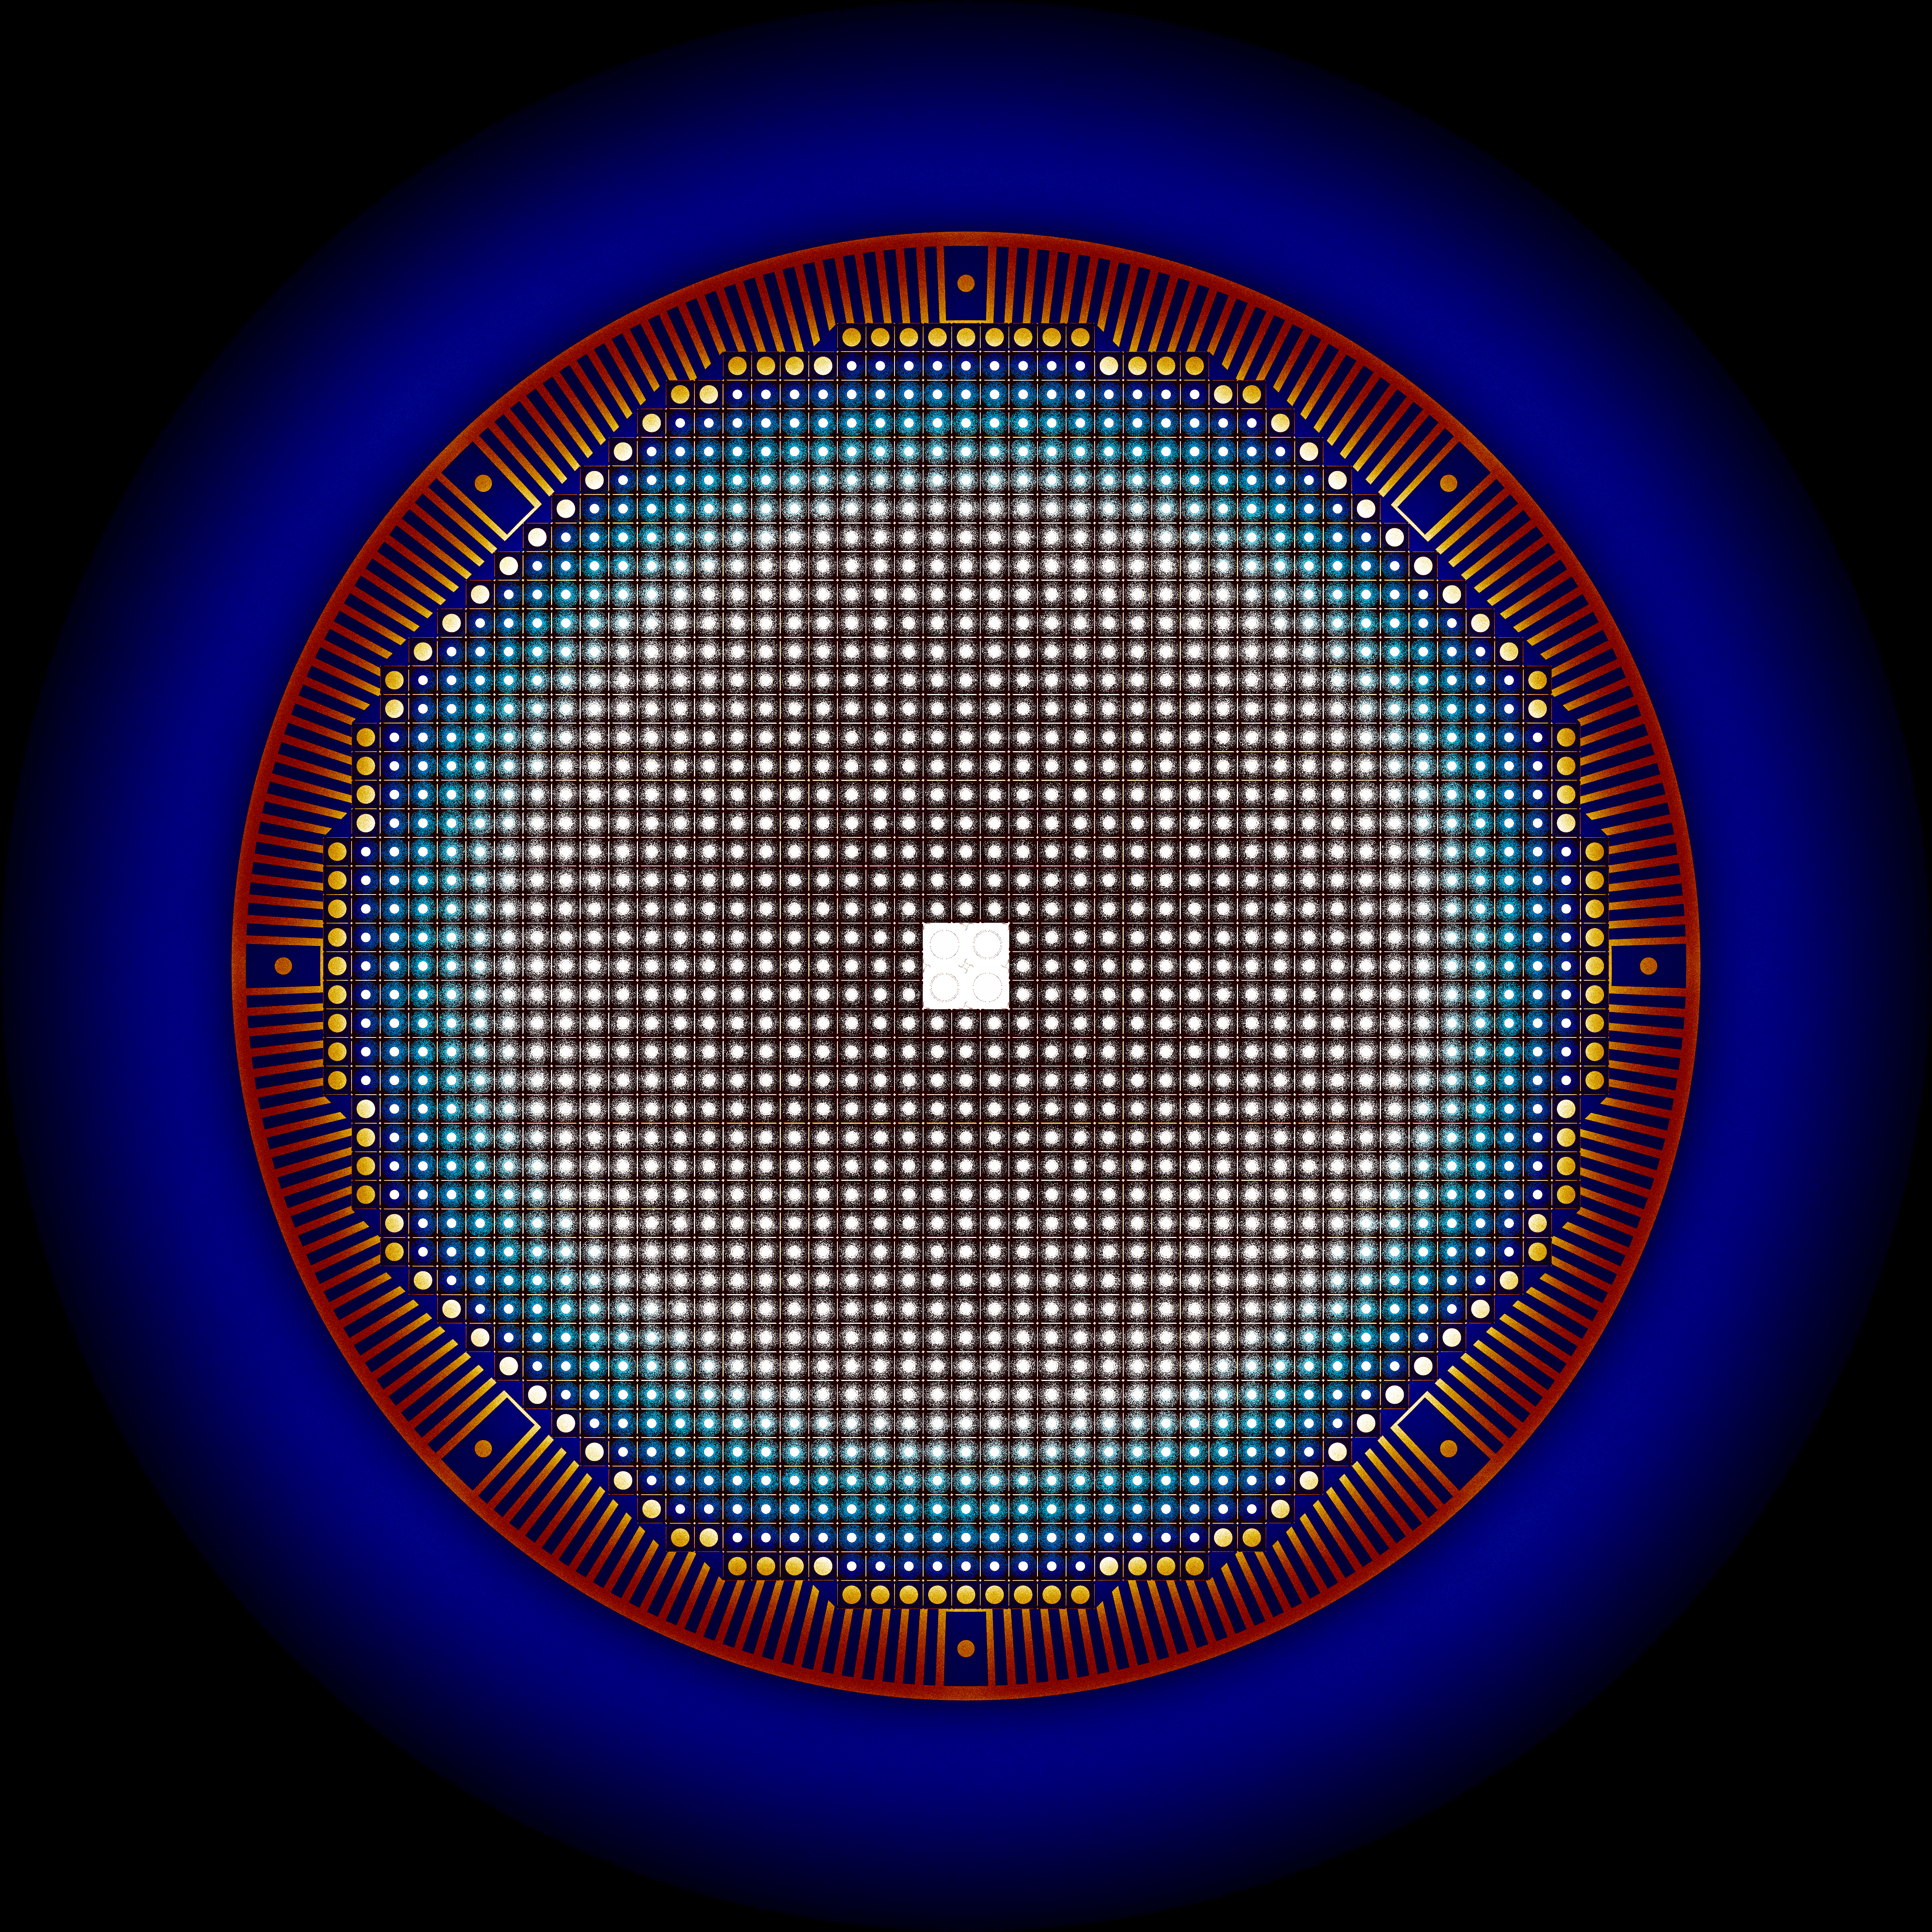
\includegraphics[height=0.71\textheight]{./images/mesh.png}
    \end{figure}
    
    \column[t]{6.5cm}
    \vspace{-0.30in}
\begin{table}[h!]
%\centering
\caption{Effective multiplication factor for full-core model}
\begin{tabular}{p{0.08\linewidth} p{0.35\linewidth} p{0.35\linewidth}} \toprule
      & SERPENT2      & Park(MCNP6)\cite{park_whole_2015}          \\ \midrule
K$_{eff}$  & 1.00397$\pm$0.00005 & 1.00736$\pm$0.00009
\\
\bottomrule
\end{tabular}
  \label{tab:keff}
       \end{table}
       
       \begin{itemize}
         \item SERPENT 2 factor is 300 pcm lower than that obtained
         by Park (MCNP6) \cite{park_whole_2015}
         \item Standard deviation is 5 pcm versus 9 pcm for Park (MCNP6) model.
       \end{itemize}

     \end{columns}
\end{frame}

\begin{frame}
  \frametitle{Effective multiplication factor for full-core model (cont.)}
   \vspace{-0.25in}
  \begin{figure}[t]
   \hspace*{-0.39in}
   \includegraphics[height=0.57\textheight]{./images/park_plan_view.png}
   \vspace{-0.05in}
   \caption{Detailed plan view of Park (MCNP6) (left) \cite{park_whole_2015}
      and SERPENT 2 (right) model.}
    \end{figure}
    \vspace{-0.15in}

    \begin{block}{Possible reasons for the discrepancy}
       \begin{itemize}
         \item Park (MCNP6) model has simplification in Zone I geometry.
         \item Zone II geometry in Park (MCNP6) has a gap between
           Zone II-A and Zone II-B.
       \end{itemize}
       \end{block}
\end{frame}

\begin{frame}
  \frametitle{Neutron spectrum}
   \vspace{-0.1in}
  \begin{figure}[t]
  % \hspace*{-0.39in}
   \includegraphics[height=0.7\textheight]{./images/spectrum.png}
   \vspace{-0.1in}
   \caption{Normalized neutron spectrum for Park(MCNP6) and SERPENT 2 model.}
    \end{figure}
    \vspace{-0.1in}

       \begin{itemize}
       \item Thermal spectrum required to breed fissile $^{233}$U from
         fertile $^{232}$Th.
       \item Hardening the spectrum tends to increased resonance absorption
         in thorium and decreased absorption in fissile material.
       \end{itemize}
\end{frame}

\begin{frame}
  \frametitle{Temperature effect of reactivity}

  The effect of temperature change on the reactivity can be expressed by temperature coefficient of reactivity:
  \begin{align}
    \alpha_T &= \frac{d\rho}{dT}
  \end{align}
  \vspace{-0.2in}
  \captionsetup[table]{
  labelsep = newline,
  name = TABLE, justification=justified,
  singlelinecheck=false,%%%%%%% a single line is centered by default
  labelsep=colon,%%%%%%
  skip = \medskipamount}

  \begin{table}[h!]
    \caption{Input data variation for temperature effect of reactivity analysis}
      \vspace{-0.1in}
  \begin{tabular}{p{0.16\linewidth} p{0.19\linewidth} p{0.27\linewidth} 
        p{0.20\linewidth}} \toprule
        $\alpha_T$ & \textbf{Nuclear data temperature} &  \textbf{Density}    & \textbf{Geometry}             \\ \midrule       
        Fuel salt        & 900-1200K & 3.28-3.13 g/cm$^3$\cite{robertson_conceptual_1971} &
        no changes\footnote{fuel salt is bounded by the graphite} \\ \midrule
        Moderator        & 900-1200K & 1.84 g/cm$^3$\cite{robertson_conceptual_1971} &
        expanded\footnote{volumes of graphite were recalculated using linear thermal expansion coefficient
           1.3$\times$10$^{-6}$ 1/K}$^{,}$\footnote{graphite density is assumed constant} \\ \midrule
        Total            & 900-1200K & fuel: 3.28-3.13g/cm$^3$ graphite: 1.84 g/cm$^3$  & only graphite expanded \\
\bottomrule
\end{tabular}
  \label{tab:tmethod}
\end{table}  
  
\end{frame}

\begin{frame}
  \frametitle{Temperature effect of reactivity (cont.)}
  \vspace{-0.1in}
  \captionsetup[table]{
  labelsep = newline,
  name = TABLE, justification=justified,
  singlelinecheck=false,%%%%%%% a single line is centered by default
  labelsep=colon,%%%%%%
  skip = \medskipamount}  
  \begin{table}[h!]
    \caption{Temperature coefficients of reactivity.}
      \vspace{-0.2in}
  \begin{tabular}{p{0.28\linewidth} p{0.22\linewidth} p{0.22\linewidth} 
        p{0.20\linewidth}} \toprule
   Reactivity coefficient [pcm/K]  & SERPENT 2      & MCNP6 
        \cite{park_whole_2015}   & Reference \cite{robertson_conceptual_1971}      
        \\ \midrule
Fuel salt        & $-3.38\pm0.015$ & $-3.20\pm0.05$ & $-3.22$ \\ \midrule
Moderator        & $+2.33\pm0.027$ & $-0.11\pm0.05$ & $+2.35$ \\ \midrule
Total            & $-1.57\pm0.033$ & $-3.21\pm0.04$ & $-0.87$ \\
\bottomrule
\end{tabular}
  \label{tab:tcoef}
\end{table}
        \begin{itemize}
       \item The fuel temperature coefficient (FTC) is negative due to
         thermal Doppler broadening of the resonance capture cross
         sections in the thorium and is in a good agreement with early research
         \cite{robertson_conceptual_1971, park_whole_2015}.
       \item The moderator temperature coefficient (MTC) is positive due to thermal expansion
         and would increase during reactor operation because of spectrum hardening along
         with fuel depletion \cite{park_whole_2015}.
       \item To obtain MTC negative and closer to MCNP6 simulation more details about
         changes in Park \emph{et al.} model needed (i.e. changes in graphite density, geometry recalculation).
       \item The isothermal temperature coefficient (ITC) is relatively large and negative and
         affords excellent reactor stability and controllability
       \end{itemize}
\end{frame}
